\documentclass[aspectratio=169, table, 12pt]{beamer}

% Preamble bersama seluruh slide mata kuliah ini.
% Dipanggil dari slides/sessionXX/sessionXX.tex tepat sesudah baris
% \documentclass[aspectratio=169, table, 12pt]{beamer}
% Paket tambahan yang hanya dibutuhkan satu sesi ditulis di berkas sesi itu.

\usepackage{colortbl}
\usepackage{xcolor}
\usepackage{listings}
\usepackage{tabularx}
\usepackage{booktabs}
\usepackage{tikz}
\usepackage{pgfplots}
\pgfplotsset{compat=1.18}
\usetikzlibrary{arrows.meta, positioning, calc, fit, shapes.geometric,
	shapes.multipart, backgrounds, matrix, chains, trees}

\makeatletter
\def\input@path{{../theme/}}
\makeatother
\graphicspath{{../theme/}{../../figures/}}
\usetheme{Pradita}

\definecolor{praditagreen}{RGB}{37, 113, 71}

% Tema membuat garis tabel berwarna putih. Dikembalikan agar tabel terbaca.
\arrayrulecolor{black}
\setlength{\arrayrulewidth}{0.5pt}

\lstdefinelanguage{yaml}{
	basicstyle=\ttfamily\scriptsize,
	keywordstyle=\color{blue}\bfseries,
	commentstyle=\color{gray}\itshape,
	stringstyle=\color{red},
	showstringspaces=false,
	breaklines=true,
	frame=lines,
	numbers=none,
	backgroundcolor=\color{lightgray!10},
	tabsize=2,
	morecomment=[l]{\#}
}

\lstdefinelanguage{json}{
	basicstyle=\ttfamily\scriptsize,
	stringstyle=\color{red},
	commentstyle=\color{gray},
	breaklines=true,
	showstringspaces=false,
	tabsize=2,
	numbers=none,
	frame=lines,
	backgroundcolor=\color{lightgray!10},
	string=[s]{"}{"}
}

\lstdefinelanguage{bash}{
	keywords={},
	basicstyle=\ttfamily\scriptsize,
	ndkeywords={docker, kubectl, helm, curl, git, terraform},
	ndkeywordstyle=\color{purple}\bfseries,
	sensitive=true,
	commentstyle=\color{gray},
	numbers=none,
	breaklines=true,
	frame=lines,
	backgroundcolor=\color{lightgray!10},
	tabsize=2,
	comment=[l]{\#},
	showstringspaces=false
}

\lstdefinelanguage{http}{
	keywords={GET, POST, PUT, PATCH, DELETE, HEAD, OPTIONS, HTTP},
	basicstyle=\ttfamily\scriptsize,
	keywordstyle=\color{blue}\bfseries,
	sensitive=true,
	numbers=none,
	breaklines=true,
	frame=lines,
	backgroundcolor=\color{lightgray!10},
	tabsize=2,
	showstringspaces=false
}

\subtitle{IT40713 · Cloud-Native \& Microservices Architecture}
\author{\textbf{Alfa Yohannis}}


\title{\Huge DevOps, GitOps, dan\\ \vspace{10pt} Platform Engineering}

\begin{document}

\frame{\titlepage}

\begin{frame}
  \frametitle{Isi Pertemuan}
  \vspace{14pt}
  \begin{columns}[t]
    \column{0.5\textwidth}
    {\small\tableofcontents[sections={1-4}]}

    \column{0.5\textwidth}
    {\small\tableofcontents[sections={5-8}]}
  \end{columns}
\end{frame}

\begin{frame}{\hfill}
  \centering
  \Huge{\textbf{Mengapa satu kolom\\baru di SIMRS\\butuh 96 hari?}}
\end{frame}

\section{Tujuan dan Konteks}

\begin{frame}{\hfill}
  \centering
  \Huge{\textbf{Tujuan dan Konteks}}
\end{frame}

\begin{frame}{{\Large Tujuan Pembelajaran}}
  \vspace{10pt}
  \begin{itemize}
    \item Menjelaskan praktik DevOps dan metrik DORA (DevOps Research and Assessment) untuk
          mengukur kinerja pengiriman perangkat lunak.
    \item Menjelaskan alur CI/CD (\textit{Continuous Integration / Continuous Delivery}) dan
          empat prinsip GitOps.
    \item Merancang topologi tim dan peran platform internal bagi organisasi.
  \end{itemize}
\end{frame}

\begin{frame}{{\Large Satu Kolom, 96 Hari}}
  \vspace{10pt}
  \begin{itemize}
    \item 15 Desember 2025: bagian pendaftaran RS Jakarta meminta kolom nomor telepon keluarga.
    \item Pemrograman diperkirakan dua hari; kolom berjalan 21 Maret 2026.
    \item Melewati tiket, dua persetujuan, antrean, uji manual, dan jendela rilis triwulanan.
    \item Waktu kerja sekitar 10 hari; 86 hari habis untuk menunggu.
    \item \textit{Cloud} dan \textit{container} tidak menolong bila alur kirimnya tetap lambat.
  \end{itemize}
\end{frame}

\IfFileExists{../../figures/ch13-diagram-konsep.png}{%
\begin{frame}{{\Large Diagram Konsep Bab 13}}
  \centering
  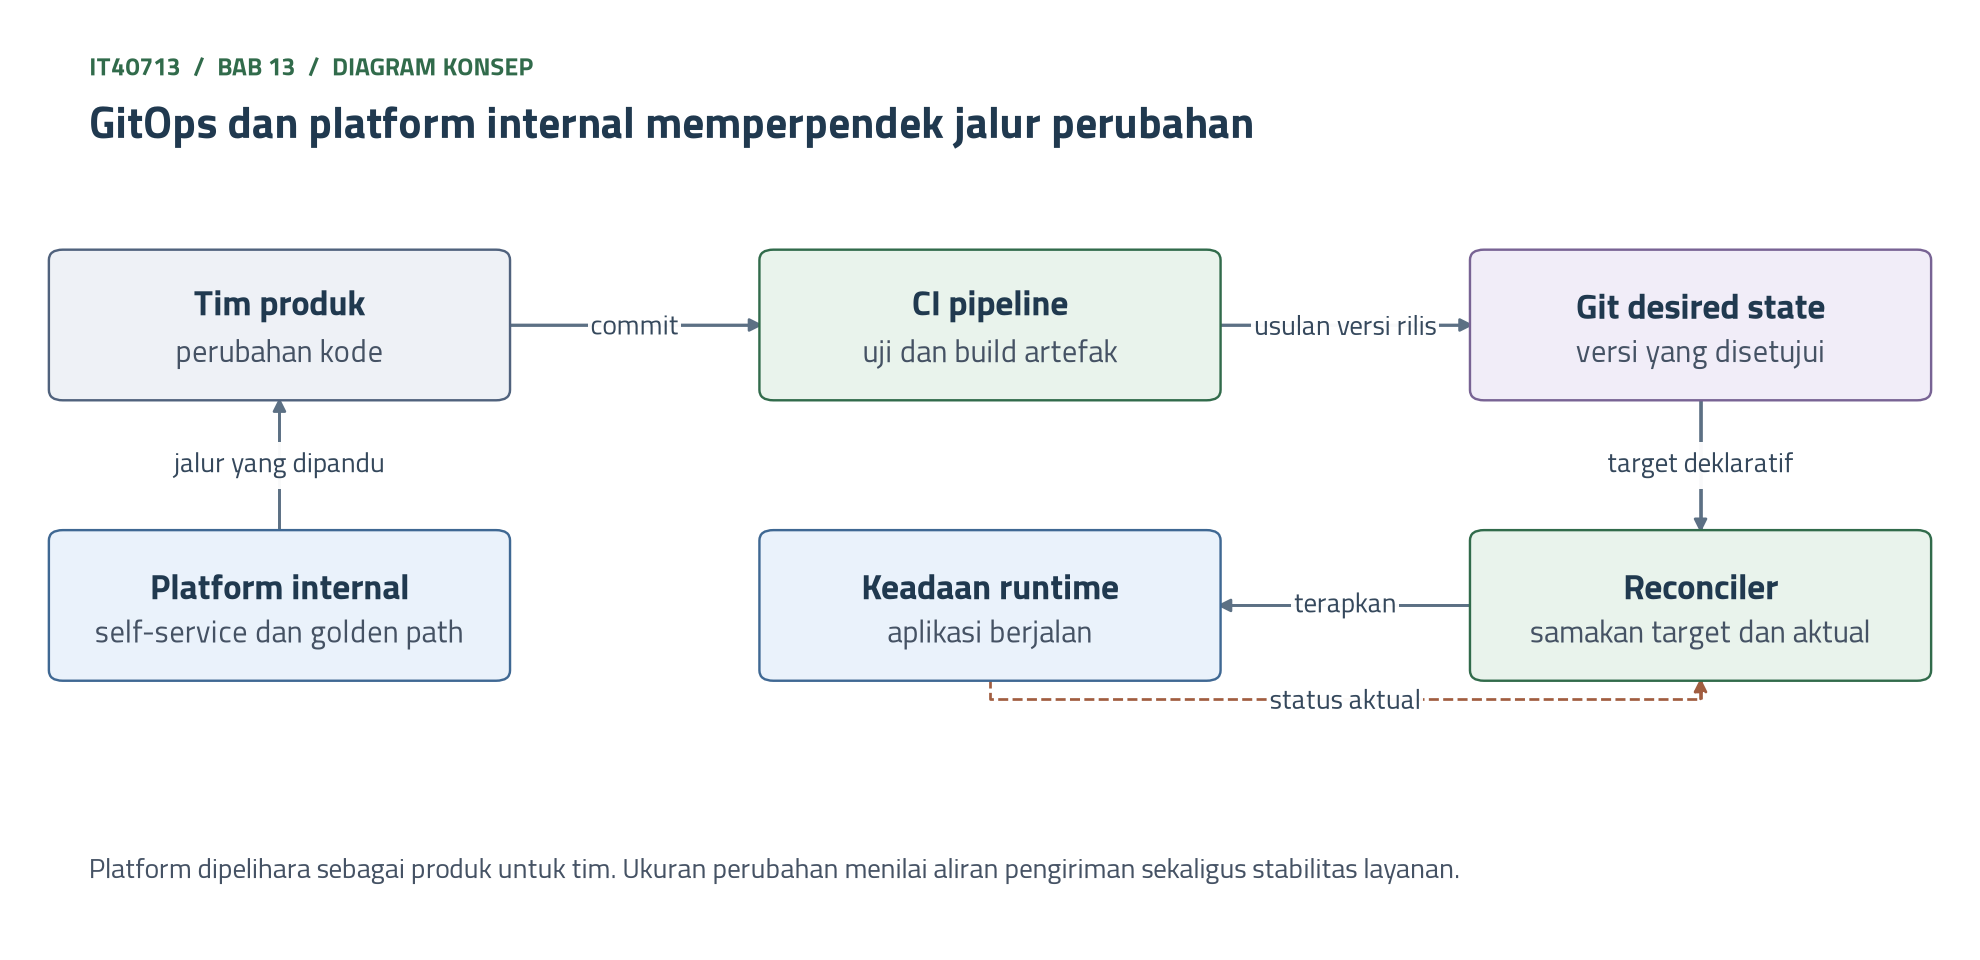
\includegraphics[width=0.96\textwidth,height=0.77\textheight,keepaspectratio]{../../figures/ch13-diagram-konsep.png}
\end{frame}
}{}

\section{DevOps dan Metrik DORA}

\begin{frame}{\hfill}
  \centering
  \Huge{\textbf{DevOps dan Metrik DORA}}
\end{frame}

\begin{frame}{{\Large DevOps sebagai Budaya dan Praktik}}
  \vspace{10pt}
  \begin{itemize}
    \item Menyatukan tanggung jawab membangun (\textit{development}) dan menjalankan
          (\textit{operations}).
    \item Bukan jabatan dan bukan alat: budaya, praktik teknis, dan praktik manajemen.
    \item Forsgren, Humble, dan Kim: 24 kapabilitas dalam lima kelompok.
    \item Contoh: 9 dari 31 permintaan pemasangan ditolak demi stabilitas, menunggu rata-rata
          47 hari.
  \end{itemize}
  \vspace{6pt}
  {\small Analogi: dapur dan ruang makan dipisah tembok; juru masak tidak pernah mendengar
  keluhan tamu.}
\end{frame}

\begin{frame}{{\Large Lima Metrik DORA}}
  \footnotesize
  \begin{tabularx}{\textwidth}{>{\raggedright\arraybackslash}p{4.6cm}
      >{\raggedright\arraybackslash}p{2.0cm} >{\raggedright\arraybackslash}X}
    \hline
    \textbf{Metrik} & \textbf{Kelompok} & \textbf{Pertanyaan yang dijawab} \\
    \hline
    \textit{Lead time} perubahan & \textit{Throughput} & Berapa lama perubahan menunggu sampai
      dipakai? \\
    \hline
    Frekuensi \textit{deployment} & \textit{Throughput} & Seberapa sering perubahan sampai ke
      pengguna? \\
    \hline
    Waktu pemulihan \textit{deployment} gagal & \textit{Throughput} & Berapa lama layanan
      terganggu? \\
    \hline
    Tingkat kegagalan perubahan & \textit{Instability} & Berapa bagian \textit{deployment} yang
      langsung butuh perbaikan? \\
    \hline
    Tingkat pengerjaan ulang & \textit{Instability} & Berapa bagian \textit{deployment} darurat
      akibat insiden? \\
    \hline
  \end{tabularx}

  \vspace{8pt}
  \small Empat yang pertama dikenal sebagai \textit{four keys}. \textit{Lead time} DORA dihitung
  sejak \textit{commit}, bukan sejak permintaan.
\end{frame}

\begin{frame}{{\Large Rilis yang Jarang Tidak Membuat Lebih Aman}}
  \footnotesize
  \begin{tabularx}{\textwidth}{>{\raggedright\arraybackslash}p{3.6cm}
      >{\raggedright\arraybackslash}X >{\raggedright\arraybackslash}p{2.6cm}
      >{\raggedright\arraybackslash}p{2.6cm}}
    \hline
    \textbf{Perubahan per rilis} & \textbf{Peluang rilis bermasalah ($p = 1$ persen)} &
      \textbf{Yang dicurigai} & \textbf{Ikut dibatalkan} \\
    \hline
    60 (triwulanan) & $1 - 0{,}99^{60} \approx 45{,}3$ persen & 60 & 59 \\
    \hline
    8 (bulanan) & $1 - 0{,}99^{8} \approx 7{,}7$ persen & 8 & 7 \\
    \hline
    1 (per perubahan) & 1 persen & 1 & 0 \\
    \hline
  \end{tabularx}

  \vspace{8pt}
  \small Riset DORA: kecepatan dan stabilitas bukan pilihan yang saling meniadakan. Analogi:
  mencuci piring setiap selesai makan, bukan menumpuknya seminggu.
\end{frame}

\begin{frame}{{\Large Temuan DORA 2025: AI sebagai Penguat}}
  \vspace{10pt}
  \begin{itemize}
    \item Survei hampir 5.000 profesional teknologi; sekitar 90 persen memakai AI.
    \item AI memperbesar kekuatan dan kelemahan yang sudah ada di organisasi.
    \item Tujuh kapabilitas dalam DORA AI Capabilities Model, tujuh profil tim.
    \item Pemrograman dua hari menjadi satu hari: \textit{lead time} hanya 96 menjadi 95 hari.
    \item Perubahan 30 persen lebih banyak: rilis 78 perubahan, peluang bermasalah 54,3 persen.
  \end{itemize}
\end{frame}

\begin{frame}{{\Large Kasus Medikara: Metrik DORA 2025}}
  \footnotesize
  \begin{tabularx}{\textwidth}{>{\raggedright\arraybackslash}p{4.4cm}
      >{\raggedright\arraybackslash}X >{\raggedright\arraybackslash}X}
    \hline
    \textbf{Metrik} & \textbf{SIMRS RS Jakarta} & \textbf{Medikara+} \\
    \hline
    \textit{Deployment} per tahun & 7 (4 terjadwal, 3 darurat) & 14 (12 terjadwal, 2 darurat) \\
    \hline
    Perubahan per rilis terjadwal & 60,5 & 7,8 \\
    \hline
    \textit{Lead time} perubahan rata-rata & 55 hari & 29 hari \\
    \hline
    Tingkat kegagalan perubahan & 3 dari 7 (43 persen) & 2 dari 14 (14 persen) \\
    \hline
    Waktu pemulihan median & 9 jam & 5 jam \\
    \hline
  \end{tabularx}

  \vspace{8pt}
  \small Yang paling jarang dirilis justru paling sering gagal. Sasaran C4: SIMRS bulanan lalu
  mingguan, gagal di bawah 15 persen, pulih di bawah satu jam.
\end{frame}

\section{CI/CD dan Strategi Rilis}

\begin{frame}{\hfill}
  \centering
  \Huge{\textbf{CI/CD dan Strategi Rilis}}
\end{frame}

\begin{frame}{{\Large Tiga Istilah yang Sering Tertukar}}
  \vspace{10pt}
  \begin{itemize}
    \item \textit{Continuous integration}: setiap penggabungan memicu \textit{build} dan uji
          otomatis.
    \item \textit{Continuous delivery}: selalu siap rilis; manusia memutuskan kapan.
    \item \textit{Continuous deployment}: lolos semua tahap, langsung ke produksi.
    \item Medikara+: 37 langkah manual (8 jam-orang) menjadi \textit{pipeline} sekitar 22 menit.
    \item Yang dibuang adalah kerja manual di sekitar persetujuan, bukan persetujuannya.
  \end{itemize}
\end{frame}

\begin{frame}{{\Large Tahap Pipeline CI/CD}}
  \centering
  \eadiagram{../../figures/ch13-pipeline-cicd.tex}
\end{frame}

\begin{frame}{{\Large Strategi Rilis}}
  \footnotesize
  \begin{tabularx}{\textwidth}{>{\raggedright\arraybackslash}p{3.2cm}
      >{\raggedright\arraybackslash}X >{\raggedright\arraybackslash}p{3.4cm}}
    \hline
    \textbf{Strategi} & \textbf{Cara kerja} & \textbf{Pembatalan} \\
    \hline
    Serentak, henti layanan & Sistem dihentikan, versi baru dipasang & Lambat, sering perlu
      pemulihan basis data \\
    \hline
    Bergilir (\textit{rolling}) & Server diganti satu per satu & Sedang \\
    \hline
    \textit{Blue-green} & Dua lingkungan identik, lalu lintas dipindah sekaligus & Cepat,
      lalu lintas dipindah kembali \\
    \hline
    \textit{Canary} & Sebagian kecil pengguna dulu, lalu diperluas & Cepat, dampak terbatas \\
    \hline
  \end{tabularx}

  \vspace{8pt}
  \small Medikara+: sekitar 933 upaya pemesanan per hari. \textit{Canary} 5 persen berarti
  sekitar 47 pemesanan; bila versi baru menggagalkan 10 persen, hanya sekitar 5 yang gagal, bukan 93.
\end{frame}

\begin{frame}{{\Large Keamanan Rantai Pasok dan Pendalaman}}
  \vspace{10pt}
  \begin{itemize}
    \item \textit{Pipeline} yang dapat memasang ke produksi juga menjadi sasaran serangan.
    \item SLSA (Supply-chain Levels for Software Artifacts): kontrol bertingkat untuk keutuhan
          paket.
    \item Kontrol awal: hak ubah \textit{pipeline} dibatasi, asal \textit{image} dapat
          dibuktikan, pustaka dipindai.
    \item Pendalaman: \textit{workflow} GitHub Actions untuk layanan jadwal dokter Bab 8.
  \end{itemize}
  \vspace{6pt}
  {\small Berkas: \berkas{sources/chapter13/contoh-pipeline-gitops/ci-jadwal-dokter.yml}}
\end{frame}

\section{Infrastructure as Code dan GitOps}

\begin{frame}{\hfill}
  \centering
  \Huge{\textbf{Infrastructure as Code\\dan GitOps}}
\end{frame}

\begin{frame}{{\Large Infrastructure as Code}}
  \vspace{10pt}
  \begin{itemize}
    \item Infrastruktur ditulis sebagai berkas, disimpan berversi, ditinjau, dan diterapkan
          otomatis.
    \item Umumnya deklaratif: menyatakan keadaan akhir, bukan urutan perintah.
    \item Lingkungan uji SIMRS: 11 hari kerja dan empat tiket menjadi sekitar 35 menit.
    \item Perubahan manual di luar berkas disebut penyimpangan (\textit{drift}).
  \end{itemize}
  \vspace{6pt}
  {\small Analogi: resep tertulis di rumah makan berjaringan; juru masak yang diam-diam menambah
  garam adalah \textit{drift}.}
\end{frame}

\begin{frame}{{\Large Empat Prinsip OpenGitOps v1.0.0}}
  \footnotesize
  \begin{tabularx}{\textwidth}{>{\raggedright\arraybackslash}p{3.8cm}
      >{\raggedright\arraybackslash}X}
    \hline
    \textbf{Prinsip} & \textbf{Arti praktis} \\
    \hline
    Deklaratif & Konfigurasi ditulis sebagai keadaan akhir \\
    \hline
    Berversi dan tidak berubah & Setiap perubahan menjadi versi baru; riwayat lengkap \\
    \hline
    Ditarik otomatis & Agen di dalam klaster mengambil perubahan dari Git \\
    \hline
    Direkonsiliasi terus & Penyimpangan terdeteksi dan dikembalikan \\
    \hline
  \end{tabularx}

  \vspace{8pt}
  \small Analogi: termostat pendingin ruangan. Yang diubah adalah angka suhu, bukan kipas
  mesinnya.
\end{frame}

\begin{frame}{{\Large Siklus GitOps}}
  \centering
  \eadiagram{../../figures/ch13-siklus-gitops.tex}
\end{frame}

\begin{frame}{{\Large Dorong, Tarik, dan Jejak Audit}}
  \vspace{10pt}
  \begin{itemize}
    \item Cara dorong: \textit{pipeline} di luar klaster memegang kunci akses produksi.
    \item Cara tarik: agen di dalam klaster mengambil perubahan dan terus merekonsiliasi.
    \item Empat bukti: \textit{commit}, tinjauan \textit{pull request}, riwayat sinkronisasi,
          laporan penyimpangan.
    \item Batas: hak tulis repositori, rahasia tidak polos di Git, akses darurat tercatat.
  \end{itemize}
\end{frame}

\begin{frame}{{\Large Kasus Medikara: Temuan Audit Kontrol Akses}}
  \vspace{10pt}
  \begin{itemize}
    \item Misalkan 17 akun memegang hak administrator langsung di server produksi.
    \item 41 perubahan konfigurasi tanpa tiket dalam enam bulan; 9 tidak tertelusuri.
    \item Usulan: hak langsung dicabut, tersisa 2 akun darurat yang ditinjau dalam 24 jam.
    \item Setiap perubahan lewat \textit{pull request} dengan dua peninjau.
    \item Biaya: perubahan darurat 15 menit, bukan 2 menit; prosedur ditulis sebelum insiden.
  \end{itemize}
\end{frame}

\section{Platform Engineering}

\begin{frame}{\hfill}
  \centering
  \Huge{\textbf{Platform Engineering}}
\end{frame}

\begin{frame}{{\Large Platform dan Internal Developer Platform}}
  \vspace{10pt}
  \begin{itemize}
    \item CNCF: kumpulan kapabilitas terpadu yang disajikan sesuai kebutuhan penggunanya.
    \item IDP (Internal Developer Platform): platform untuk tim pengembang di dalam organisasi.
    \item \textit{Golden path}: templat proyek awal beserta dokumentasinya.
    \item \textit{Self-service} dan \textit{platform as a product}: diukur dari pemakaian.
    \item \textit{Golden path} untuk layanan stok obat: 14 hari menjadi satu hari.
  \end{itemize}
  \vspace{6pt}
  {\small Analogi: dapur bersama yang menyewakan kompor, gudang pendingin, dan izin higienis.}
\end{frame}

\begin{frame}{{\Large Lapisan Platform Internal Medikara}}
  \centering
  \eadiagram{../../figures/ch13-lapisan-platform.tex}
\end{frame}

\begin{frame}{{\Large Tim Platform Bukan Loket Tiket}}
  \footnotesize
  \begin{tabularx}{\textwidth}{>{\raggedright\arraybackslash}p{3.4cm}
      >{\raggedright\arraybackslash}X >{\raggedright\arraybackslash}X}
    \hline
    \textbf{Aspek} & \textbf{Divisi berbasis tiket} & \textbf{Tim platform} \\
    \hline
    Cara melayani & Permintaan satu per satu & Kapabilitas swalayan dipakai berulang \\
    \hline
    Satuan kerja & Tiket & Produk internal dengan peta jalan \\
    \hline
    Ukuran keberhasilan & Tiket selesai & Adopsi, kepuasan, metrik DORA pengguna \\
    \hline
    Bila permintaan naik & Antrean memanjang & Biaya per pemakaian turun \\
    \hline
  \end{tabularx}

  \vspace{8pt}
  \small Mulai dari \textit{thinnest viable platform}; platform dipakai karena memudahkan, bukan
  karena diwajibkan.
\end{frame}

\begin{frame}{{\Large Platform Engineering Maturity Model}}
  \footnotesize
  \begin{tabularx}{\textwidth}{>{\raggedright\arraybackslash}p{2.0cm}
      >{\raggedright\arraybackslash}X >{\raggedright\arraybackslash}X
      >{\raggedright\arraybackslash}X >{\raggedright\arraybackslash}X}
    \hline
    \textbf{Aspek} & \textbf{1. \textit{Provisional}} & \textbf{2. \textit{Operationalized}} &
      \textbf{3. \textit{Scalable}} & \textbf{4. \textit{Optimizing}} \\
    \hline
    Investasi & Sukarela & Tim khusus & Didanai sebagai produk & Ekosistem \\
    \hline
    Adopsi & Tidak menentu & Didorong perintah & Ditarik nilai & Pengguna berkontribusi \\
    \hline
    Antarmuka & Proses manual & \textit{Golden path} & Swalayan & Menyatu dengan alat kerja \\
    \hline
    Operasi & Bila diminta & Punya pemilik & Proses baku & Siklus hidup otomatis \\
    \hline
    Pengukuran & Seadanya & Konsisten & Wawasan & Kuantitatif dan kualitatif \\
    \hline
  \end{tabularx}

  \vspace{8pt}
  \small Medikara: tingkat 1 di semua aspek; sasaran dua tahun tingkat 2, antarmuka tingkat 3.
\end{frame}

\section{Team Topologies}

\begin{frame}{\hfill}
  \centering
  \Huge{\textbf{Team Topologies}}
\end{frame}

\begin{frame}{{\Large Empat Tipe Tim dan Tiga Mode Interaksi}}
  \vspace{10pt}
  \begin{itemize}
    \item \textit{Stream-aligned}: mengirim perubahan untuk satu aliran nilai (tim bangsal).
    \item Platform: layanan internal swalayan (instalasi sterilisasi pusat).
    \item \textit{Enabling}: melatih tim lain lalu mundur; \textit{complicated-subsystem}:
          keahlian langka.
    \item Mode: \textit{collaboration}, \textit{X-as-a-Service}, \textit{facilitating}.
    \item Ukurannya beban kognitif tim; kaitannya dengan hukum Conway (Bab 7).
  \end{itemize}
\end{frame}

\begin{frame}{{\Large Topologi Tim Target Medikara}}
  \centering
  \eadiagram{../../figures/ch13-topologi-tim-medikara.tex}
\end{frame}

\begin{frame}{{\Large Kasus Medikara: Dari Tim per Rumah Sakit}}
  \vspace{10pt}
  \begin{itemize}
    \item 52 staf TI: 26 di rumah sakit (12 pengembang), 26 di kantor pusat.
    \item 15 staf pusat pindah: platform 6, Medikara+ 4, integrasi FHIR 3, \textit{enabling} 2.
    \item Beban kognitif turun: dari sembilan modul per rumah sakit menjadi dua sampai tiga modul
          per tim.
    \item Risiko: tim \textit{enabling} dan integrasi di bawah ukuran tim yang dianjurkan.
    \item Tanpa \textit{self-service}, enam orang tim platform kembali menjadi loket tiket.
  \end{itemize}
\end{frame}

\section{Aktivitas}

\begin{frame}{{\Large Aktivitas: Model Operasi Delivery}}
  \vspace{10pt}
  \begin{enumerate}
    \item Petakan alur satu perubahan kecil dari permintaan sampai produksi.
    \item Tandai antrean dan langkah manual; hitung efisiensi alur dan metrik DORA.
    \item Rancang alur CI/CD dan GitOps target; persetujuan yang tersisa diberi alasan risiko.
    \item Susun topologi tim target dan mode interaksinya.
    \item Pilih tiga sampai lima kapabilitas platform beserta urutannya.
  \end{enumerate}
\end{frame}

\begin{frame}{{\Large Contoh Pemetaan Alur: Kolom Nomor Telepon Keluarga}}
  \footnotesize
  \begin{tabularx}{\textwidth}{>{\raggedright\arraybackslash}X
      >{\raggedleft\arraybackslash}p{2.0cm} >{\raggedleft\arraybackslash}p{2.0cm}}
    \hline
    \textbf{Langkah} & \textbf{Proses (hari)} & \textbf{Tunggu (hari)} \\
    \hline
    Tiket, persetujuan kepala instalasi, komite bulanan & 1,5 & 31 \\
    \hline
    Antre menunggu pengembang & 0 & 20 \\
    \hline
    Pemrograman dan tinjauan kode & 2 & 3 \\
    \hline
    Uji fungsional dan uji regresi manual & 6 & 32 \\
    \hline
    Rilis Sabtu malam, henti layanan 4 jam & 0,5 & 0 \\
    \hline
    \textbf{Jumlah} (\textit{lead time} 96 hari, efisiensi 10,4 persen) & \textbf{10} &
      \textbf{86} \\
    \hline
  \end{tabularx}
\end{frame}

\begin{frame}{{\Large Peran, Luaran, dan Penilaian}}
  \vspace{10pt}
  \begin{itemize}
    \item Non-teknis: memimpin pemetaan waktu tunggu dan rantai persetujuan.
    \item Teknis: merancang alur CI/CD dan GitOps, menghitung metrik DORA.
    \item Luaran C4: model operasi \textit{delivery} dan peta jalan platform internal.
    \item Bobot: pemetaan 30, alur target 25, topologi 25, peta jalan 20 persen.
    \item Templat: \berkas{sources/chapter13/templat-model-operasi-delivery.md}
  \end{itemize}
\end{frame}

\section{Ringkasan dan Latihan}

\begin{frame}{{\Large Ringkasan}}
  \vspace{10pt}
  \begin{itemize}
    \item Rilis jarang berukuran besar, lebih sering gagal, dan lebih lama dipulihkan.
    \item AI adalah penguat: perbaikan berarti ada di alur kerja, bukan di alatnya.
    \item CI/CD, \textit{blue-green}, dan \textit{canary} memperkecil rilis dan risiko.
    \item GitOps membuat jejak audit siapa mengubah apa dari kerja sehari-hari.
    \item Tim platform dan Team Topologies menurunkan beban kognitif tim pengirim nilai.
  \end{itemize}
\end{frame}

\begin{frame}{{\Large Latihan}}
  \vspace{10pt}
  \begin{enumerate}
    \item Organisasi yang merilis perubahan setiap tiga bulan sering menganggap rilis yang
          jarang lebih aman. Kritisi anggapan ini dengan merujuk temuan DORA.
    \item Apa perbedaan tim platform dengan divisi infrastruktur tradisional yang melayani
          tiket?
    \item Jelaskan cara GitOps membantu auditor menelusuri siapa mengubah apa di lingkungan
          produksi.
  \end{enumerate}
\end{frame}

\end{document}
